\documentclass[12pt]{article}
%Fall 2022
% Some basic packages
\usepackage{standalone}[subpreambles=true]
\usepackage[utf8]{inputenc}
\usepackage[T1]{fontenc}
\usepackage{textcomp}
\usepackage[english]{babel}
\usepackage{url}
\usepackage{graphicx}
%\usepackage{quiver}
\usepackage{float}
\usepackage{enumitem}
\usepackage{lmodern}
\usepackage{comment}
\usepackage{hyperref}
\usepackage[usenames,svgnames,dvipsnames]{xcolor}
\usepackage[margin=1in]{geometry}
\usepackage{pdfpages}

\pdfminorversion=7

% Don't indent paragraphs, leave some space between them
\usepackage{parskip}

% Hide page number when page is empty
\usepackage{emptypage}
\usepackage{subcaption}
\usepackage{multicol}
\usepackage[b]{esvect}

% Math stuff
\usepackage{amsmath, amsfonts, mathtools, amsthm, amssymb}
\usepackage{bbm}
\usepackage{stmaryrd}
\allowdisplaybreaks

% Fancy script capitals
\usepackage{mathrsfs}
\usepackage{cancel}
% Bold math
\usepackage{bm}
% Some shortcuts
\newcommand{\rr}{\ensuremath{\mathbb{R}}}
\newcommand{\zz}{\ensuremath{\mathbb{Z}}}
\newcommand{\qq}{\ensuremath{\mathbb{Q}}}
\newcommand{\nn}{\ensuremath{\mathbb{N}}}
\newcommand{\ff}{\ensuremath{\mathbb{F}}}
\newcommand{\cc}{\ensuremath{\mathbb{C}}}
\newcommand{\ee}{\ensuremath{\mathbb{E}}}
\newcommand{\hh}{\ensuremath{\mathbb{H}}}
\renewcommand\O{\ensuremath{\emptyset}}
\newcommand{\norm}[1]{{\left\lVert{#1}\right\rVert}}
\newcommand{\dbracket}[1]{{\left\llbracket{#1}\right\rrbracket}}
\newcommand{\ve}[1]{{\bm{#1}}}
\newcommand\allbold[1]{{\boldmath\textbf{#1}}}
\DeclareMathOperator{\lcm}{lcm}
\DeclareMathOperator{\im}{im}
\DeclareMathOperator{\coim}{coim}
\DeclareMathOperator{\dom}{dom}
\DeclareMathOperator{\tr}{tr}
\DeclareMathOperator{\rank}{rank}
\DeclareMathOperator*{\var}{Var}
\DeclareMathOperator*{\ev}{E}
\DeclareMathOperator{\dg}{deg}
\DeclareMathOperator{\aff}{aff}
\DeclareMathOperator{\conv}{conv}
\DeclareMathOperator{\inte}{int}
\DeclareMathOperator*{\argmin}{argmin}
\DeclareMathOperator*{\argmax}{argmax}
\DeclareMathOperator{\graph}{graph}
\DeclareMathOperator{\sgn}{sgn}
\DeclareMathOperator*{\Rep}{Rep}
\DeclareMathOperator{\Proj}{Proj}
\DeclareMathOperator{\mat}{mat}
\DeclareMathOperator{\diag}{diag}
\DeclareMathOperator{\aut}{Aut}
\DeclareMathOperator{\gal}{Gal}
\DeclareMathOperator{\inn}{Inn}
\DeclareMathOperator{\edm}{End}
\DeclareMathOperator{\Hom}{Hom}
\DeclareMathOperator{\ext}{Ext}
\DeclareMathOperator{\tor}{Tor}
\DeclareMathOperator{\Span}{Span}
\DeclareMathOperator{\Stab}{Stab}
\DeclareMathOperator{\cont}{cont}
\DeclareMathOperator{\Ann}{Ann}
\DeclareMathOperator{\Div}{div}
\DeclareMathOperator{\curl}{curl}
\DeclareMathOperator{\nat}{Nat}
\DeclareMathOperator{\gr}{Gr}
\DeclareMathOperator{\vect}{Vect}
\DeclareMathOperator{\id}{id}
\DeclareMathOperator{\Mod}{Mod}
\DeclareMathOperator{\sign}{sign}
\DeclareMathOperator{\Surf}{Surf}
\DeclareMathOperator{\fcone}{fcone}
\DeclareMathOperator{\Rot}{Rot}
\DeclareMathOperator{\grad}{grad}
\DeclareMathOperator{\atan2}{atan2}
\DeclareMathOperator{\Ric}{Ric}
\let\vec\relax
\DeclareMathOperator{\vec}{vec}
\let\Re\relax
\DeclareMathOperator{\Re}{Re}
\let\Im\relax
\DeclareMathOperator{\Im}{Im}
% Put x \to \infty below \lim
\let\svlim\lim\def\lim{\svlim\limits}

%wide hat
\usepackage{scalerel,stackengine}
\stackMath
\newcommand*\wh[1]{%
\savestack{\tmpbox}{\stretchto{%
  \scaleto{%
    \scalerel*[\widthof{\ensuremath{#1}}]{\kern-.6pt\bigwedge\kern-.6pt}%
    {\rule[-\textheight/2]{1ex}{\textheight}}%WIDTH-LIMITED BIG WEDGE
  }{\textheight}% 
}{0.5ex}}%
\stackon[1pt]{#1}{\tmpbox}%
}
\parskip 1ex

%Make implies and impliedby shorter
\let\implies\Rightarrow
\let\impliedby\Leftarrow
\let\iff\Leftrightarrow
\let\epsilon\varepsilon

% Add \contra symbol to denote contradiction
\usepackage{stmaryrd} % for \lightning
\newcommand\contra{\scalebox{1.5}{$\lightning$}}

% \let\phi\varphi

% Command for short corrections
% Usage: 1+1=\correct{3}{2}

\definecolor{correct}{HTML}{009900}
\newcommand\correct[2]{\ensuremath{\:}{\color{red}{#1}}\ensuremath{\to }{\color{correct}{#2}}\ensuremath{\:}}
\newcommand\green[1]{{\color{correct}{#1}}}

% horizontal rule
\newcommand\hr{
    \noindent\rule[0.5ex]{\linewidth}{0.5pt}
}

% hide parts
\newcommand\hide[1]{}

% si unitx
\usepackage{siunitx}
\sisetup{locale = FR}

%allows pmatrix to stretch
\makeatletter
\renewcommand*\env@matrix[1][\arraystretch]{%
  \edef\arraystretch{#1}%
  \hskip -\arraycolsep
  \let\@ifnextchar\new@ifnextchar
  \array{*\c@MaxMatrixCols c}}
\makeatother

\renewcommand{\arraystretch}{0.8}

\renewcommand{\baselinestretch}{1.5}

\usepackage{graphics}
\usepackage{epstopdf}

\RequirePackage{hyperref}
%%
%% Add support for color in order to color the hyperlinks.
%% 
\hypersetup{
  colorlinks = true,
  urlcolor = blue,
  citecolor = blue
}
%%fakesection Links
\hypersetup{
    colorlinks,
    linkcolor={red!50!black},
    citecolor={green!50!black},
    urlcolor={blue!80!black}
}
%customization of cleveref
\RequirePackage[capitalize,nameinlink]{cleveref}[0.19]

% Per SIAM Style Manual, "section" should be lowercase
\crefname{section}{section}{sections}
\crefname{subsection}{subsection}{subsections}
\Crefname{section}{Section}{Sections}
\Crefname{subsection}{Subsection}{Subsections}

% Per SIAM Style Manual, "Figure" should be spelled out in references
\Crefname{figure}{Figure}{Figures}

% Per SIAM Style Manual, don't say equation in front on an equation.
\crefformat{equation}{\textup{#2(#1)#3}}
\crefrangeformat{equation}{\textup{#3(#1)#4--#5(#2)#6}}
\crefmultiformat{equation}{\textup{#2(#1)#3}}{ and \textup{#2(#1)#3}}
{, \textup{#2(#1)#3}}{, and \textup{#2(#1)#3}}
\crefrangemultiformat{equation}{\textup{#3(#1)#4--#5(#2)#6}}%
{ and \textup{#3(#1)#4--#5(#2)#6}}{, \textup{#3(#1)#4--#5(#2)#6}}{, and \textup{#3(#1)#4--#5(#2)#6}}

% But spell it out at the beginning of a sentence.
\Crefformat{equation}{#2Equation~\textup{(#1)}#3}
\Crefrangeformat{equation}{Equations~\textup{#3(#1)#4--#5(#2)#6}}
\Crefmultiformat{equation}{Equations~\textup{#2(#1)#3}}{ and \textup{#2(#1)#3}}
{, \textup{#2(#1)#3}}{, and \textup{#2(#1)#3}}
\Crefrangemultiformat{equation}{Equations~\textup{#3(#1)#4--#5(#2)#6}}%
{ and \textup{#3(#1)#4--#5(#2)#6}}{, \textup{#3(#1)#4--#5(#2)#6}}{, and \textup{#3(#1)#4--#5(#2)#6}}

% Make number non-italic in any environment.
\crefdefaultlabelformat{#2\textup{#1}#3}

% Environments
\makeatother
% For box around Definition, Theorem, \ldots
%%fakesection Theorems
\usepackage{thmtools}
\usepackage[framemethod=TikZ]{mdframed}

\theoremstyle{definition}
\mdfdefinestyle{mdbluebox}{%
	roundcorner = 10pt,
	linewidth=1pt,
	skipabove=12pt,
	innerbottommargin=9pt,
	skipbelow=2pt,
	nobreak=true,
	linecolor=blue,
	backgroundcolor=TealBlue!5,
}
\declaretheoremstyle[
	headfont=\sffamily\bfseries\color{MidnightBlue},
	mdframed={style=mdbluebox},
	headpunct={\\[3pt]},
	postheadspace={0pt}
]{thmbluebox}

\mdfdefinestyle{mdredbox}{%
	linewidth=0.5pt,
	skipabove=12pt,
	frametitleaboveskip=5pt,
	frametitlebelowskip=0pt,
	skipbelow=2pt,
	frametitlefont=\bfseries,
	innertopmargin=4pt,
	innerbottommargin=8pt,
	nobreak=false,
	linecolor=RawSienna,
	backgroundcolor=Salmon!5,
}
\declaretheoremstyle[
	headfont=\bfseries\color{RawSienna},
	mdframed={style=mdredbox},
	headpunct={\\[3pt]},
	postheadspace={0pt},
]{thmredbox}

\declaretheorem[%
style=thmbluebox,name=Theorem,numberwithin=section]{thm}
\declaretheorem[style=thmbluebox,name=Lemma,sibling=thm]{lem}
\declaretheorem[style=thmbluebox,name=Proposition,sibling=thm]{prop}
\declaretheorem[style=thmbluebox,name=Corollary,sibling=thm]{coro}
\declaretheorem[style=thmredbox,name=Example,sibling=thm]{eg}

\mdfdefinestyle{mdgreenbox}{%
	roundcorner = 10pt,
	linewidth=1pt,
	skipabove=12pt,
	innerbottommargin=9pt,
	skipbelow=2pt,
	nobreak=true,
	linecolor=ForestGreen,
	backgroundcolor=ForestGreen!5,
}

\declaretheoremstyle[
	headfont=\bfseries\sffamily\color{ForestGreen!70!black},
	bodyfont=\normalfont,
	spaceabove=2pt,
	spacebelow=1pt,
	mdframed={style=mdgreenbox},
	headpunct={ --- },
]{thmgreenbox}

\declaretheorem[style=thmgreenbox,name=Definition,sibling=thm]{defn}

\mdfdefinestyle{mdgreenboxsq}{%
	linewidth=1pt,
	skipabove=12pt,
	innerbottommargin=9pt,
	skipbelow=2pt,
	nobreak=true,
	linecolor=ForestGreen,
	backgroundcolor=ForestGreen!5,
}
\declaretheoremstyle[
	headfont=\bfseries\sffamily\color{ForestGreen!70!black},
	bodyfont=\normalfont,
	spaceabove=2pt,
	spacebelow=1pt,
	mdframed={style=mdgreenboxsq},
	headpunct={},
]{thmgreenboxsq}
\declaretheoremstyle[
	headfont=\bfseries\sffamily\color{ForestGreen!70!black},
	bodyfont=\normalfont,
	spaceabove=2pt,
	spacebelow=1pt,
	mdframed={style=mdgreenboxsq},
	headpunct={},
]{thmgreenboxsq*}

\mdfdefinestyle{mdblackbox}{%
	skipabove=8pt,
	linewidth=3pt,
	rightline=false,
	leftline=true,
	topline=false,
	bottomline=false,
	linecolor=black,
	backgroundcolor=RedViolet!5!gray!5,
}
\declaretheoremstyle[
	headfont=\bfseries,
	bodyfont=\normalfont\small,
	spaceabove=0pt,
	spacebelow=0pt,
	mdframed={style=mdblackbox}
]{thmblackbox}

\theoremstyle{plain}
\declaretheorem[name=Question,sibling=thm,style=thmblackbox]{ques}
\declaretheorem[name=Remark,sibling=thm,style=thmgreenboxsq]{remark}
\declaretheorem[name=Remark,sibling=thm,style=thmgreenboxsq*]{remark*}
\newtheorem{ass}[thm]{Assumptions}

\theoremstyle{definition}
\newtheorem*{problem}{Problem}
\newtheorem{claim}[thm]{Claim}
\theoremstyle{remark}
\newtheorem*{case}{Case}
\newtheorem*{notation}{Notation}
\newtheorem*{note}{Note}
\newtheorem*{motivation}{Motivation}
\newtheorem*{intuition}{Intuition}
\newtheorem*{conjecture}{Conjecture}

% Make section starts with 1 for report type
%\renewcommand\thesection{\arabic{section}}

% End example and intermezzo environments with a small diamond (just like proof
% environments end with a small square)
\usepackage{etoolbox}
\AtEndEnvironment{vb}{\null\hfill$\diamond$}%
\AtEndEnvironment{intermezzo}{\null\hfill$\diamond$}%
% \AtEndEnvironment{opmerking}{\null\hfill$\diamond$}%

% Fix some spacing
% http://tex.stackexchange.com/questions/22119/how-can-i-change-the-spacing-before-theorems-with-amsthm
\makeatletter
\def\thm@space@setup{%
  \thm@preskip=\parskip \thm@postskip=0pt
}

% Fix some stuff
% %http://tex.stackexchange.com/questions/76273/multiple-pdfs-with-page-group-included-in-a-single-page-warning
\pdfsuppresswarningpagegroup=1


% My name
\author{Jaden Wang}



\begin{document}
\centerline {\textsf{\textbf{\LARGE{Homework 4}}}}
\centerline {Jaden Wang}
\vspace{.15in}
\begin{problem}[1]
\begin{enumerate}[label=(\alph*)]
The Hamiltonian of the problem is given by
\begin{align*}
	H(x_1,x_2,u,p_1,p_2) = \frac{1}{2} u ^2+ p_1x_2+p_2(u-x_2). 
\end{align*}
The adjoint equations are given by
\begin{align*}
	\dot{p_1} &= -H_{x_1} = 0 \\
	\dot{p_2} &= -H_{x_2} = p_2-p_1 .
\end{align*}
The first-order condition demands
\begin{align*}
	H_u = u+p_2 &= 0\\
	u&= -p_2 .
\end{align*}
Plugging this into the differential equations yield
\begin{align*}
	\dot{x_1} &= x_2 \\
	\dot{x_2} &= -x_2-p_2 .
\end{align*}
Together with the adjoint equations, we have 4 first-order equations and require 4 boundary conditions.
\item Since all initial and final times and states are fixed, we have 4 boundary conditions $ x_1(0)=x_2(0)=0$, $ x_1(3)=1$, and $ x_2(3)=2$. Mathematica yields
\begin{align*}
	u(t) &= \frac{6e^{3+t}+6e^{t}-e^{6}+4e^{3}-3}{e^{6}+4e^{3}-5}\\
	&=-0.6811 + 0.2642 e^{t}.
\end{align*}
~\begin{figure}[H]
	\centering
	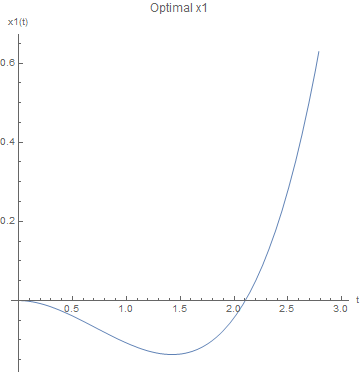
\includegraphics[width=0.3\textwidth]{./figures/4.1.png}
	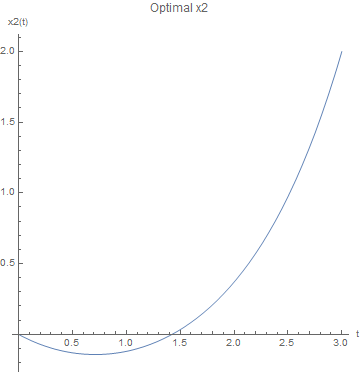
\includegraphics[width=0.3\textwidth]{./figures/4.2.png}
	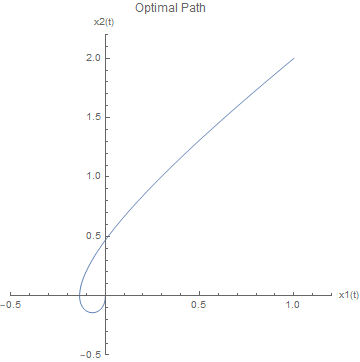
\includegraphics[width=0.3\textwidth]{./figures/4.3.png}
\end{figure}
\item When $ x_2(3)$ is free, in its place we instead have the transversality condition $ p_2(3) = 0$. This yields the solution
\begin{align*}
	u(t) &= -\frac{2e^3(e^{t}-e^{3})}{3e^{6}+4e^3-1 }\\
	&= 0.6256 - 0.0311e^{t} \\
\end{align*}
~\begin{figure}[H]
	\centering
	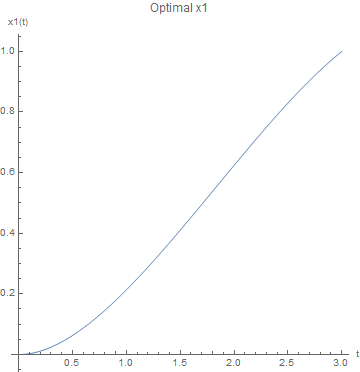
\includegraphics[width=0.3\textwidth]{./figures/4.4.png}
	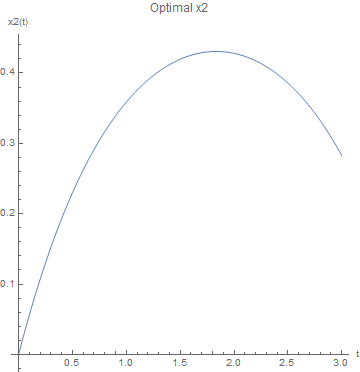
\includegraphics[width=0.3\textwidth]{./figures/4.5.png}
	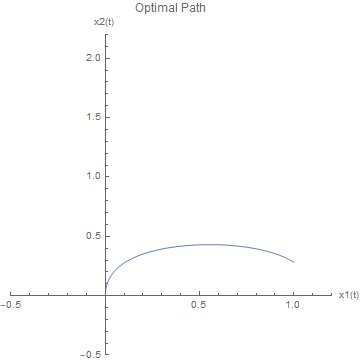
\includegraphics[width=0.3\textwidth]{./figures/4.6.png}
\end{figure}

\item I would add a final penalty term $ \Phi$:
\begin{align*}
	\mathcal{ J} = \underbrace{ \frac{1}{2} \left( (x_1(3)-1)^2+(x_2(3)-2)^2 \right)  }_{\Phi(3) } + \frac{1}{2} \int_0^3 u^2 dt .
\end{align*}
Then instead of $ p_1(3)=p_2(3)=0$, we have
\begin{align*}
	p_1(3) &= \Phi_{x_1}(3) = x_1(3)-1 \\
	p_2(3) &= \Phi_{x_2}(3) = x_2(3)-2 
\end{align*}
Then new control is
\begin{align*}
	u(t) &= \frac{8e^{3+t}+6e^{t}+e^{6}+4e^3-3}{7e^{6}+8e^3-7}\\
	&= 0.1615+0.056 e^{t} .
\end{align*}
~\begin{figure}[H]
	\centering
	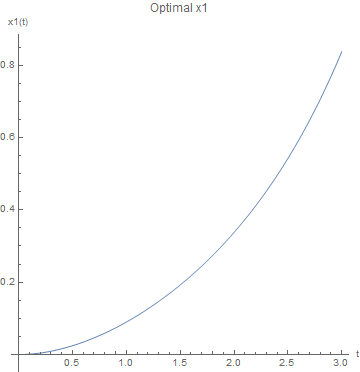
\includegraphics[width=0.3\textwidth]{./figures/4.7.png}
	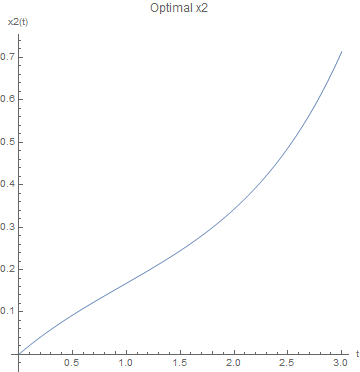
\includegraphics[width=0.3\textwidth]{./figures/4.8.png}
	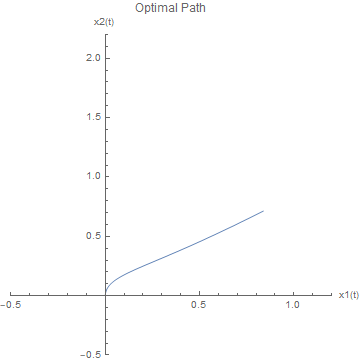
\includegraphics[width=0.3\textwidth]{./figures/4.9.png}
\end{figure}
We see that $ x_1(3) = 0.8385$ and $ x_2(3) = 0.7142$, which are not very close to $ (1,2)$. To improve accuracy, I would increase the weight of the penalty term. We see that the cost in part (a) is  $ 4.2859$. The cost as a function of the weight coefficient  $ c$ is shown in the figure below:
~\begin{figure}[H]
	\centering
	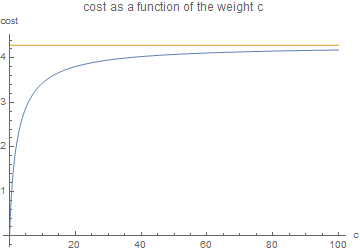
\includegraphics[width=0.4\textwidth]{./figures/4.10.png}
	\caption{We see that as the weight increases, the cost approaches that of the cost (orange) in part (a) asymptotically.}
\end{figure}
And we indeed see that the solution ends much closer to $ (1,2)$ when the weight is high:
~\begin{figure}[H]
	\centering
	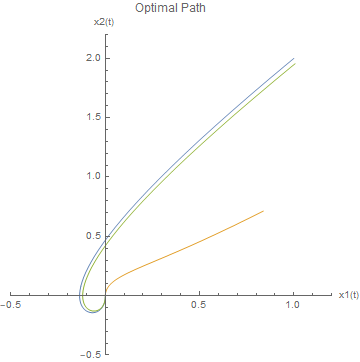
\includegraphics[width=0.4\textwidth]{./figures/4.11.png}
	\caption{Blue is optimal path from part (a), green is part (c) with weight 100, and orange is part (c) with weight 1.}
\end{figure}

\item It is clear that $ \Psi = \begin{pmatrix} 2&5 \end{pmatrix} $. By transversality condition from Equation 5.234, we have the boundary conditions
\begin{align*}
	\begin{pmatrix} -p_1(3)\\-p_2(3) \end{pmatrix} &= \begin{pmatrix} 2\\5 \end{pmatrix} \lambda 
\end{align*}
Together with the initial conditions $ x_1(0)=x_2(0)=0$ and the terminal condition $ 2 x_1(3) + 5x_2(3) = 20$, we have 5 boundary conditions for 4 differential equations and an unknown $ \lambda$. This allows us to solve by Mathematica and obtain the optimal control:
\begin{align*}
	u(t)=-p_2(t)= 1.4341+0.1071 e^{t}
\end{align*}
~\begin{figure}[H]
	\centering
	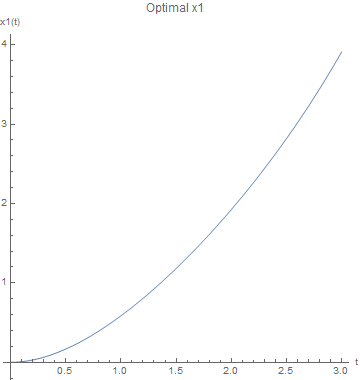
\includegraphics[width=0.3\textwidth]{./figures/4.12.png}
	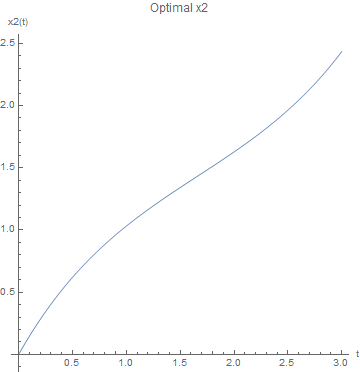
\includegraphics[width=0.3\textwidth]{./figures/4.13.png}
	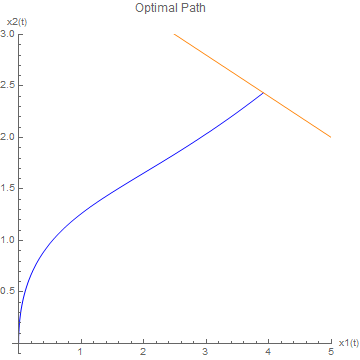
\includegraphics[width=0.3\textwidth]{./figures/4.14.png}
	\caption{We see that the solution indeed ends at the constraint.}
\end{figure}

\item We have the same $\Psi $ but $ h(t) = 20 +\frac{t^2}{ 2}$ so $ \dot{h}(t_f) = t_f$. When $ t_f$ is also free, based on Equation 5.234 we have the transversality conditions
\begin{align*}
	\begin{pmatrix} H(t_f)\\ -p_1(t_f)\\-p_2(t_f) \end{pmatrix} &= \begin{pmatrix} -t_f\\ 2\\5 \end{pmatrix} \lambda 
\end{align*}
Note that by plugging in $ u=-p_2$, we have
\begin{align*}
	H &= -\frac{1}{2} p_2^2+(p_1-p_2)x_2\\
	H(t_f)&= -\frac{25}{2} \lambda + 3x_2(t_f) = -t_f 
\end{align*}
Together with two initial conditions and the terminal condition
\begin{align*}
	2x_1(t_f) +5x_2(t_f) = 20 + \frac{t_f^2}{ 2},
\end{align*}
we have a total of 6 boundary conditions to match the 4 differential equations and two unknowns $ \lambda$ and $ t_f$. Mathematica yields
\begin{align*}
	u(t) = 1.8359 + 0.2547 e^{t} .
\end{align*}
The trajectories are
~\begin{figure}[H]
	\centering
	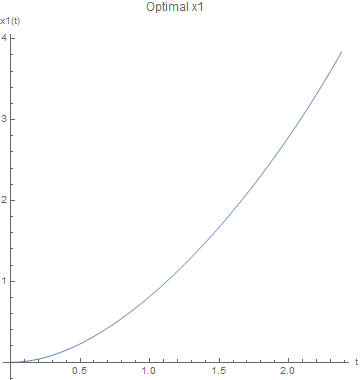
\includegraphics[width=0.3\textwidth]{./figures/4.15.png}
	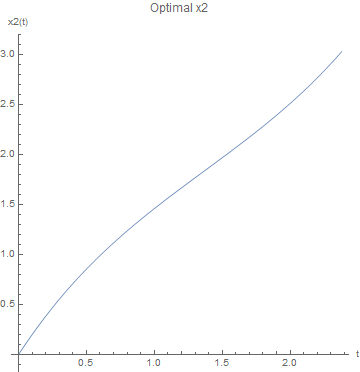
\includegraphics[width=0.3\textwidth]{./figures/4.16.png}
	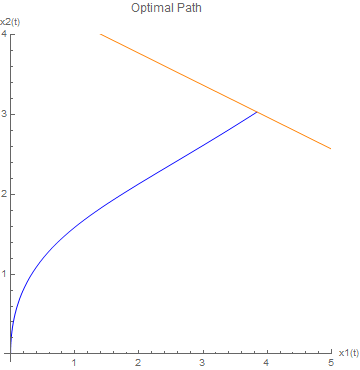
\includegraphics[width=0.3\textwidth]{./figures/4.17.png}
	\caption{We see the end point hits the constraint.}
\end{figure}
\end{enumerate}
\end{problem}
\begin{problem}[2]
The Hamiltonian is
\begin{align*}
	H = \frac{1}{2} u^2 + p(ax+bu)
\end{align*}
The adjoint equation is
\begin{align*}
	\dot{p} = -H_x = ap \implies p(t) = C e^{at}.
\end{align*}
And the first-order condition is
\begin{align*}
	H_u = u+bp = 0 \implies u=-bp
\end{align*}
Thus
\begin{align*}
	\dot{x} = ax-b^2p = ax - b^2 C e^{at}, \quad x(0)=x_0,x(tf) = 0
\end{align*}
We have $ x(t) = b^2 C t e^{at} + A e^{at}$, $ x(0) = A = x_0$, and
\begin{align*}
	x(t_f) = b^2 C t_f e^{at_f} + x_0 e^{at_f} &= 0 \\
	C &= - \frac{x_0}{ b^2 t_f}
\end{align*}
Thus,
\begin{align*}
	u(t) = -bp = -b \cdot \left( - \frac{x_0}{b^2 t_f} \right) e^{at}  = \frac{x_0}{ b t_f} e^{at}
\end{align*}
\end{problem}
\begin{problem}[3]
With the mixed constraint $ \psi(x_0,x_f) = x_f - x_0 = 0$, we can turn $ x_0,x_f$ into free variables by adding a term with Lagrange multiplier. Let $ \Phi(x_0,x_f) = \phi(x_f) + \lambda \psi(x_0,x_f)= \frac{1}{2}(x(t_f)-1)^2 + \lambda(x_f - x_0)$. The Hamiltonian is
\begin{align*}
	H = \frac{1}{2} (x^2+u^2)+pu .
\end{align*}
The adjoint equation is
\begin{align*}
	\dot{p}= -H_x = x
\end{align*}
The first-order condition says
\begin{align*}
	H_u = u +p=0 \implies u = -p .
\end{align*}
Since both $x(0), x(2)$ is free, from Equation 5.234 we have the transversality condition
 \begin{align*}
	 (\Phi_{x_0}+p ^{T}(t_0)) \delta x_0 + (\Phi_{x_f}- p ^{T}(t_f)	\delta x_f = 0
\end{align*}
where $ \delta x_0$ and $ \delta x_f$ can take any value. This forces that
\begin{align*}
	\Phi_{x_0} + p ^{T}(t_0) &=0 \\
	\Phi_{x_f} - p ^{T}(t_f) &= 0 
\end{align*}
Thus for this problem, we have
\begin{align*}
	p(0) &= -\Phi_{x_0} = -(- \lambda ) = \lambda\\
	p(2) &= \Phi_{x_f} = x(2) -1 + \lambda  
\end{align*}

Thus we have two boundary conditions for two differential equations. Mathematica yields
\begin{align*}
	x(t) = \frac{\lambda \cos (2-t) + \cos t - \lambda \cost t + \lambda \sin (2-t)}{ \cos 2 - \sin 2 }.
\end{align*}
Solving $ x(0) = x(2)$, we obtain  $ \lambda = \frac{\cos(2)-1}{ 2 \cos 2 + \sin 2-2} \approx 0.7364$.
\begin{align*}
	u(t) &= -p(t) = \frac{\lambda (\cos(2-t)-\sin(2-t)-\sin t)+ \sin t}{\cos 2 - \sin 2 }\\
	&= 0.5556 (\cos(2-t)-\sin(2-t)) + 0.1989 \sin t
\end{align*}
The associated cost is $ 1.8506$.
\end{problem}

\begin{problem}[4]
\begin{enumerate}[label=(\alph*)]
\item Since the cost $ \mathcal{ J} = t_f$, we have $ \Phi(t) = t$ and the Hamiltonian is
	\begin{align*}
		H= p_1(t) \cos \theta (t) + p_2(t) \sin \theta(t) + p_3(t) u(t) + p_4(t) v(t)
	\end{align*}
\item The adjoint equations are
\begin{align*}
	\begin{pmatrix} \dot{p_1}\\\dot{p_2}\\\dot{p_3}\\ \dot{p_4} \end{pmatrix} = \begin{pmatrix} -H_u\\-H_v\\-H_x\\-H_y \end{pmatrix} = \begin{pmatrix} p_3\\p_4\\0\\0 \end{pmatrix} 
\end{align*}
\item Since $ t_f, u(t_f),v(t_f)$ are free, by Equation 5.234 we have  the transversality conditions
	\begin{align*}
		H(t_f) + \Phi_t(t_f) = 0 \implies H(t_f) = -1 \\
		p_1(t_f) = \Phi_u = 0\\
		p_2(t_f) = \Phi_v = 0 .
	\end{align*}
\item Notice that $ p_3,p_4$ are constants, so $ p_1(t) = p_3t$ and $ p_2(t) = p_4t$ by the zero boundary conditions. First-order condition yields
\begin{align*}
	H_\theta = -p_1 \sin \theta(t) + p_2 \cos \theta(t) &= 0 \\
	\tan \theta^*(t)  &= \frac{p_2(t)}{ p_1(t)} = \frac{p_4}{ p_3}
\end{align*}
which is a constant! So are $ \cos \theta^* $ and $ \sin \theta^* $. Thus by the initial conditions $u(0)= \cos \gamma_0, v(0) = \sin \gamma_0$, we have $ u(t) = \cos \theta^* t$ and $ v(t) = \sin \theta^* $. By the initial conditions $x(0)=y(0)=0$, we have $ x(t) = \frac{1}{2} \cos \theta^* t^2 + \cos \gamma_0 t$ and $ y(t) = \frac{1}{2} \sin \theta^* t^2+ \sin \gamma_0 t$. By the terminal condition $ x(t_f)=x_f$ and  $ y(t_f)=0$, we have 
\begin{align*}
	x_f -\cos \gamma_0 t_f &= \frac{1}{2} \cos \theta^* t_f^2\\
	- \sin \gamma_0 t_f &= \frac{1}{2} \sin \theta^* t_f^2 
\end{align*}
Squaring both sides and adding the two equations together, we obtain the equation as desired:
\begin{align*}
	x_f^2-2\cos \gamma_0 t_f + (\cos \gamma_0^2+\sin \gamma_0^2) t_f^2 &= \frac{1}{4} (\cos^2\theta^* +\sin^2\theta^* )t_f^{4}\\
	4x_f^2-8 \cos \gamma_0 t_f + 4t_f^2 - t_f^{4} &= 0 
\end{align*}
So $ t_f$ must be the minimum positive solution of this equation.
\item By the above equation,
\begin{align*}
	\cos \theta^* &= 2\left(\frac{x_f}{t_f^2}+\frac{\cos \gamma_0}{ t_f}\right) \\
	\theta^* &= \arccos \left( 2\left(\frac{x_f}{t_f^2}+\frac{\cos \gamma_0}{ t_f^}\right)  \right)  
\end{align*}
\end{enumerate}
\end{problem}
\begin{problem}[5]
The cost has the Meyer form $ J = t_f$ so  $ \Phi(t) = t$. The Hamiltonian is
\begin{align*}
	H(x,y,p_1,p_2) &= p_1 r \cos \beta + p_2 r \sin \beta .
\end{align*}
The adjoint equations are
\begin{align*}
	\dot{p_1} &= -H_x = - p_1 \frac{x}{r} \cos \beta - p_2 \frac{x}{r} \sin \beta \\
	\dot{p_2} &= -H_y = p_1 \frac{y}{r} \cos \beta - p_2 \frac{x}{r} \sin \beta 
\end{align*}
Note that $ \dot{p_2} = \frac{y}{x} \dot{p_1}$. First-order condition yields
\begin{align*}
	H_{\beta} = -p_1 r \sin \beta + p_2 r \cos \beta &= 0 \\
	\tan \beta &= \frac{p_2}{p_1} 
\end{align*}
Thus we obtain $ p_2 = \tan \beta p_1$. Moreover, we see that
\begin{align*}
	p_2 \cos \beta - p_1 \sin \beta &= \frac{p_2p_1 - p_1 p_2}{ \sqrt{p_1^2+p_2^2} } \\
	&= 0 .
\end{align*}
Now we compute
\begin{align*}
	0=\frac{d}{dt} H_{ \beta} &= \dot{r} (-p_1 \sin \beta + p_2 \cos \beta) + r\left( -\frac{d}{dt}(p_1 \sin \beta) + \frac{d}{dt}(p_2 \cos \beta) \right)  \\
				0&=0 + r \left( -\dot{p_1} \sin \beta - p1 \cos \beta \dot{\beta} + \dot{p_2} \cos \beta - p_2 \sin \beta \dot{\beta} \right)   \\
				0&= -\dot{p_1} \sin \beta - p1 \cos \beta \dot{\beta} + \frac{y}{x} \dot{p_1} \cos \beta - p_1\tan \beta \sin \beta \dot{\beta} \\
				p_1 (cos \beta + \tan \beta \sin \beta) \dot{ \beta} &= \dot{p_1} \left( - \sin \beta + \frac{y}{x} \cos \beta \right)  \\
				p_1 (cos \beta + \tan \beta \sin \beta) \dot{ \beta} &= \left( p_1 \frac{x}{r} \cos \beta + \tan \beta p_1 \frac{x}{r} \sin \beta \right)  \left( \sin \beta - \frac{y}{x} \cos \beta \right)  \\
				\dot{\beta}&= \frac{x}{r} \left( \sin \beta - \frac{y}{x} \cos \beta \right)  \\
				\dot{\beta} &=  \frac{x}{r} sin \beta - \frac{y}{r} \cos \beta
\end{align*}
\end{problem}
\end{document}
